\documentclass[11pt]{article}
\usepackage{graphicx}
\usepackage{fullpage}
\usepackage{amsmath,amsthm,amsfonts,amssymb,amscd}
\usepackage{lipsum}
\usepackage{titlesec}
\usepackage{longtable}
\usepackage[top=0.6in,bottom=1in,left=0.8in,right=0.8in]{geometry}
\usepackage[utf8]{inputenc}
\usepackage{listings}
\usepackage{xcolor}
\usepackage{verbatim}
\usepackage{setspace}
\usepackage[colorlinks,allcolors={blue}]{hyperref}

% don't indent paragraphs 
\setlength{\parindent}{0pt}
% inter-paragraph spacing
\setlength{\parskip}{1em}
% line spacing
\setstretch{1.25}

\definecolor{codegreen}{rgb}{0,0.6,0}
\definecolor{codegray}{rgb}{0.5,0.5,0.5}
\definecolor{codepurple}{rgb}{0.58,0,0.82}
\definecolor{backcolour}{rgb}{0.95,0.95,0.92}

\lstdefinestyle{mystyle}{
    backgroundcolor=\color{backcolour},   
    commentstyle=\color{codegreen},
    keywordstyle=\color{magenta},
    numberstyle=\tiny\color{codegray},
    stringstyle=\color{codepurple},
    basicstyle=\ttfamily\footnotesize,
    breakatwhitespace=false,         
    breaklines=true,                 
    captionpos=b,                    
    keepspaces=true,                 
    numbers=left,                    
    numbersep=5pt,                  
    showspaces=false,                
    showstringspaces=false,
    showtabs=false,                  
    tabsize=2
}
 
\lstset{style=mystyle}

% title formatting
\titleformat{\section}
{\centering\normalfont\scshape}{\thesection.}{1em}{}
\titleformat{\subsection}
{\centering\normalfont\scshape}{\thesubsection.}{1em}{}

% spacing between columns
% \setlength{\columnsep}{2em}

%title setup
\title{\vspace{-1cm}Introductory Exercise: Ohm's Law\\[0.4cm]\large{PHY224H1 S | Winter 2020}\vspace{-0.5em}}
\author{Jeff Shen}
\date{\vspace{-0.3em}\normalsize17 January 2020}

%%%%%%%%%%%%%%%%%%%%%%%%%%%%%%%%%%%
\begin{document}

\maketitle

\section{Introduction}

The purpose of this exercise is to investigate how current, voltage, and resistance are related by Ohm's Law. We vary the voltage and see how that changes the current in a circuit. We then use these values to calculate resistance (with errors propagated through), and compare this to reference values. 

\section{Setup}

The setup of the circuit was as follows:
\begin{itemize}
    \item negative terminal of the power supply connected to the common terminal  of multimeter \#1
    \item ammeter terminal of multimeter \#1 connected to one side of the resistor
    \item the same side of the resistor also connected to the common terminal of multimeter \#2
    \item voltage/resistance terminal of multimeter \#2 connected to other side of the resistor
    \item the same side of the resistor also connected to the positive terminal of the power supply
\end{itemize}

\begin{figure}[htb]
    \centering 
    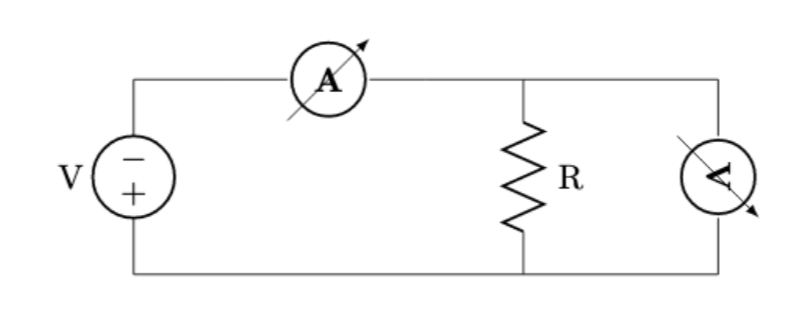
\includegraphics[width=0.5\linewidth]{circuit.png}
    \caption{\label{fig:circuit}Circuit diagram of setup.}
\end{figure}

\section{Method}

\begin{enumerate}
    \item Connect setup to resistor.
    \item Turn on power supply and both multimeters.
    \item Record the voltage. 
    \item Change the voltage. 
\end{enumerate}

Set the lower portion of one multimeter to DCA (the ammeter) and the other to DCV (the voltmeter). The upper portions of the ammeter and the voltmeter are set to the lowest settings which still give a readout (in order to get the most digits possible). In most cases, the voltmeter should be at the 20V setting, and the ammeter will use the 2mA, 20mA, and 200mA settings.

Select four resistors (blue-grey-brown-gold, green-orange-brown-gold, orange-orange-orange-gold, and grey-orange-red-gold). Start with one, and, repeat steps 3-4 a total of ten times. Disconnect the setup, and complete steps 1-4 for each of the other three resistors. There should be 40 data points. 

Afterwards, disassemble the setup. Take one of the multimeters, and use it to measure the resistance for each of the four resistors. Connect one side of the resistor to the common terminal of the multimeter, and the other to the voltage/resistance terminal. Set the lower portion of the multimeter to read the resistance. Set the upper portion, again, to the lowest setting which gives a readable output. This is the 2 kiloohm setting for the blue-grey-brown-gold and the green-orange-brown-gold resistors, the 20 kiloohm setting for the grey-orange-red-gold resistor, and the 200 kiloohm setting for the orange-orange-orange-gold resistor.

\section{Data}


\begin{table}[!htb]
    \caption{Data for grey-orange-brown-gold resistor.}
    \vspace{1em}\hline\hline\vspace{0.3em}\centering
    \begin{tabular}{cccc}
        Current (mA)&Current Uncertainty (mA)&Voltage (V)&Voltage Uncertainty (V)\\
        \hline
1.373 mA&0.010 mA&1.122 V&0.003 V\\
3.81 mA&0.03 mA&3.11 V&0.01 V\\
6.30 mA&0.05 mA&5.12 V&0.01 V\\
6.82 mA&0.05 mA&5.53 V&0.01 V\\
9.36 mA&0.07 mA&7.60 V&0.02 V\\
9.49 mA&0.07 mA&7.72 V&0.02 V\\
14.22 mA&0.10 mA&11.56 V&0.03 V\\
15.57 mA&0.11 mA&12.67 V&0.03 V\\
17.07 mA&0.13 mA&13.83 V&0.03 V\\
19.36 mA&0.15 mA&15.64 V&0.04 V\\

    \end{tabular}
    \hline\hline
\end{table}


\begin{table}[!htb]
    \caption{Data for orange-orange-orange-gold resistor.}
    \vspace{1em}\hline\hline\vspace{0.3em}\centering
    \begin{tabular}{cccc}
        Current (mA)&Current Uncertainty (mA)&Voltage (V)&Voltage Uncertainty (V)\\
        \hline
0.131 mA&0.001 mA&4.42 V&0.01 V\\
0.170 mA&0.001 mA&5.57 V&0.01 V\\
0.187 mA&0.001 mA&6.23 V&0.02 V\\
0.232 mA&0.002 mA&7.74 V&0.02 V\\
0.301 mA&0.002 mA&10.06 V&0.03 V\\
0.345 mA&0.003 mA&11.54 V&0.03 V\\
0.401 mA&0.003 mA&13.41 V&0.03 V\\
0.456 mA&0.003 mA&15.23 V&0.04 V\\
0.518 mA&0.004 mA&17.37 V&0.04 V\\
0.585 mA&0.004 mA&19.55 V&0.05 V\\

    \end{tabular}
    \hline\hline
\end{table}

\begin{table}[!htb]
    \caption{Data for blue-grey-brown-gold resistor.}
    \vspace{1em}\hline\hline\vspace{0.3em}\centering
    \begin{tabular}{cccc}
        Current (mA)&Current Uncertainty (mA)&Voltage (V)&Voltage Uncertainty (V)\\
        \hline

1.96 mA&0.01 mA&1.33 V&0.01 V\\
7.34 mA&0.06 mA&4.96 V&0.01 V\\
8.22 mA&0.06 mA&5.50 V&0.01 V\\
10.77 mA&0.08 mA&7.27 V&0.02 V\\
11.50 mA&0.09 mA&7.76 V&0.02 V\\
14.35 mA&0.11 mA&9.67 V&0.02 V\\
16.89 mA&0.13 mA&11.38 V&0.03 V\\
18.55 mA&0.14 mA&12.45 V&0.03 V\\
23.8 mA&0.2 mA&15.97 V&0.04 V\\
26.2 mA&0.2 mA&17.50 V&0.04 V\\

    \end{tabular}
    \hline\hline
\end{table}


\begin{table}[!htb]
    \caption{Data for blue-grey-brown-gold resistor.}
    \vspace{1em}\hline\hline\vspace{0.3em}\centering
    \begin{tabular}{cccc}
        Current (mA)&Current Uncertainty (mA)&Voltage (V)&Voltage Uncertainty (V)\\
        \hline

0.518 mA&0.004 mA&4.34 V&0.01 V\\
0.675 mA&0.005 mA&5.58 V&0.01 V\\
0.785 mA&0.006 mA&6.49 V&0.02 V\\
0.926 mA&0.007 mA&7.65 V&0.02 V\\
1.060 mA&0.008 mA&8.77 V&0.02 V\\
1.382 mA&0.010 mA&11.43 V&0.03 V\\
1.448 mA&0.011 mA&11.97 V&0.03 V\\
1.666 mA&0.012 mA&13.78 V&0.03 V\\
1.869 mA&0.015 mA&15.48 V&0.04 V\\
2.13 mA&0.02 mA&17.6 V&0.04 V\\

    \end{tabular}
    \hline\hline
\end{table}

Uncertainties are calculated by taking the largest of the error of accuracy and error of precision. Error of accuracy is taken to be percentages of the reading, according to the multimeter setting. For the percentages, consult the multimeter specifications \href{https://faraday.physics.utoronto.ca/specs/tegam130a.html}{here}. Where necessary, round the uncertainty to match the decimal place of the measurement. 

\newpage
\section{Results}

Using the voltage and the current, we calculate the resistance of each resistor following Ohm's Law:
\begin{alignat*}{2}
    &&V &= IR \\
    \implies&&R &= \frac{V}{I} \\
\end{align*}
Since our measurements for current were all done in mA, we need to divide them by 1000 to ensure that units are consistent (A, V, $\Omega$). 

So, for each resistor, we have 10 resistance calculations. Then, we calculate the average calculated resistances according to the formula 
\begin{align*}
    \overline{R} = \frac{1}{10}\sum_{i=1}^{10}R_i.
\end{align*}

The standard error is calculated as 
\begin{align*}
    SE = \frac{s}{\sqrt{10}},
\end{align*}
where 
\begin{align*}
    s = \sqrt{\frac{\sum_{i=1}^{10}(R_i - \overline{R})^2}{9}}.
\end{align*}

The measurement uncertainty was again the maximum of the uncertainty in accuracy and precision, where the uncertainty in accuracy is taken from the specifications of the multimeter as a percentage of the reading. 

\begin{table}[htb]
    \caption{Calculated, measured, and read resistances compared.}
    \vspace{1em}\hline\hline\vspace{0.3em}\centering
    \begin{tabular}{ccccccc}
        &Average Calculated&Standard&Measured&Measurement&Colour Band&Tolerance\\
        &Resistance&Error&Resistance&Uncertainty&Resistance&\\
        \hline
        grey-orange-&813 $\Omega$&.3 $\Omega$&814 $\Omega$&2 $\Omega$&830 $\Omega$&42 $\Omega$ \\
        -brown-gold&&&&&& \\
        orange-orange-&33384 $\Omega$&25 $\Omega$&33400 $\Omega$&66.8 $\Omega$&33000 $\Omega$&1650 $\Omega$ \\
        -orange-gold&&&&&& \\
        blue-grey-&673.1 $\Omega$&.3 $\Omega$&675 $\Omega$& 1 $\Omega$&680 $\Omega$&34 $\Omega$ \\
        -brown-gold&&&&&& \\
        blue-grey-&8280.1 $\Omega$&3.5 $\Omega$&8270 $\Omega$&17 $\Omega$&8300 $\Omega$&415 $\Omega$ \\
        -brown-gold&&&&&& \\
    \end{tabular}
    \hline\hline
\end{table}

\section{Sources of Uncertainty}

We did not carry out the experiment as described above. We started with the resistor that has the colour bands blue-grey-brown-gold. We repeated steps 1-3 for each of the resistors. Then, we changed the voltage, and repeated steps 1-3 for each of the resistors again. We did this a total of three times. So, we had three data points for each of the seven resistors. At this point, we realized that we needed to have a lot of data points for a few resistors rather than a few points for a lot of resistors. So, we conducted another round of data collection. We followed the procedure described above, but rather than 10 data points, we collected 7 for each of the 4 resistors. So, we had 10 data points (3+7) for four resistors, and 3 data points for three resistors. So, including the three data points collected earlier, we had a total of 10 data points for these four resistors. We decided not to include the data for the other three resistors. Since we disconnected the setup in between the two rounds of data collection, there may be some 

Furthermore, before the experiment started, one of our multimeters broke, and we switched it out. The multimeter might be a source of uncertainty, whether it be because of additional resistance or fluctutations in readings. 

\section{Conclusion}

In this lab, we set out to investigate the relationship between current, voltage, and resistance. By repeatedly taking measurements of voltage and current using different resistors, we found that for a fixed resistance, current and voltage have a positive linear relationship. We practiced propagating errors throughout our calculations, and found that most of our measurements were within acceptable parameters. 

\end{document}
